\documentclass[usepdftitle=false,10pt]{beamer}
\usetheme{Dresden}
\usepackage{amsmath}
\usepackage{mathrsfs}
\usepackage{amssymb}
\usepackage{xcolor}
\usepackage{multirow}
\usepackage{subcaption}

\usepackage{enumitem}
\newlist{mylist}{itemize}{2}
\setlist[mylist]{label=$\square$}


\usepackage{pifont}
\newcommand{\cmark}{\color{green} \ding{51}}%
\newcommand{\xmark}{\color{red} \ding{55}}%
\newcommand{\done}{\rlap{$\square$}{\raisebox{2pt}{\large\hspace{1pt}\cmark}}%
\hspace{-2.5pt}}
\newcommand{\wontfix}{\rlap{$\square$}{\large\hspace{1pt}\xmark}}

% Mathematical Shortcuts
\newcommand{\pfrac}[2]{\frac{\partial #1}{\partial #2}}   % partial derivative
\newcommand{\difrac}[2]{\frac{d #1}{d #2}}                % derivative
\newcommand{\bpar}[1]{\left( #1 \right)}                  % big parentheses
\newcommand{\bbra}[1]{\left[ #1 \right]}                  % big brackets
\newcommand{\bbar}[1]{\left| #1 \right|}                  % big bars
\newcommand{\bra}[1]{\left\langle #1 \right\vert}         % bra
\newcommand{\ket}[1]{\left\vert #1 \right\rangle}         % ket
\newcommand{\inner}[2]{\left\langle #1 \left\vert\right. #2 \right\rangle}            % bracket
\newcommand{\innerop}[3]{\left\langle #1 \left\vert #2 \right\vert #3 \right\rangle}  % operator matrix element
\newcommand{\innersub}[4]{\langle \bd{#1}_{#2}, \bd{#3}_{#4} \rangle}                 % bracket with subscripts
\newcommand{\half}{\frac{1}{2}}                           % 1/2
\newcommand{\powfrac}[3]{\bpar{\frac{#1}{#2}}^{#3}}       % fraction raised to a power
\newcommand{\ii}{\infty}                                  % infinity symbol
\newcommand{\tquad}{\quad\quad\quad}                      % triple-quad spacing
\renewcommand{\Im}{\text{Im}}                             % imaginary symbol
\renewcommand{\Re}{\text{Re}}                             % real symbol

\newcommand*\mycommand[1]{\texttt{\emph{#1}}}
\newcommand*\suchthat[0]{\text{ }\vert\text{ }}
\newcommand*\complexmatfield[1]{\mathbb{C}^{#1\text{x}#1}}
\newcommand*\speciallinear[2]{\mathrm{UnL}(#1,#2)}
\newcommand*\complexspeciallinear[1]{\speciallinear{#1}{\mathbb{C}}}
\newcommand*\generallinear[2]{\mathrm{GL}(#1,#2)}
\newcommand*\complexgenerallinear[1]{\generallinear{#1}{\mathbb{C}}}
\newcommand*\mat[1]{\boldsymbol{#1}}

\newcommand*\vc[1]{\boldsymbol{#1}}
\newcommand*\op[1]{\mathcal{#1}}

% Redo iint
\renewcommand*\iint[0]{\int\hspace{-8pt}\int}

\newcommand\blfootnote[1]{%
  \begingroup
  \renewcommand\thefootnote{}\footnote{#1}%
  \addtocounter{footnote}{-1}%
  \endgroup
}

\renewcommand*\footnoterule{}

\title{Modeling Spin--Forbidden Processes via Explicit Treatment of \emph{ab initio} Relativistic Effects in Non--Adiabatic Dynamics}
\date{Wednesday, October 19, 2016, 10:00 AM \\ CHB 239}
\author{David Williams-Young\\ Department of Chemistry, University of Washington\\
}

\begin{document}

% Title Page
\begin{frame}
  \titlepage
\end{frame}

% Talk outline
\begin{frame}
  \frametitle{Outline}
  \begin{itemize}
    \item[\ding{228}] Motivation: Spin--Forbidden Processes
    \item[\ding{228}] Solution: Relativistic Non--Adiabatic Molecular Dynamics
%    \item Trajectory Surface Hopping
%    \item[\ding{228}] Relativistic Theory Primer
%    \item The Configuration Interaction Method
    \item[\ding{228}] Previous Work
    \item[\ding{228}] Future Directions
  \end{itemize}
\end{frame}

% What is ISC
\begin{frame}
  \frametitle{Spin--Forbidden Processes: Intersystem Crossing (ISC)}

  \noindent
  Intersystem crossing is characterized by an electronic transition between
  quantum states of differing spin multiplicity.

  \begin{center}
  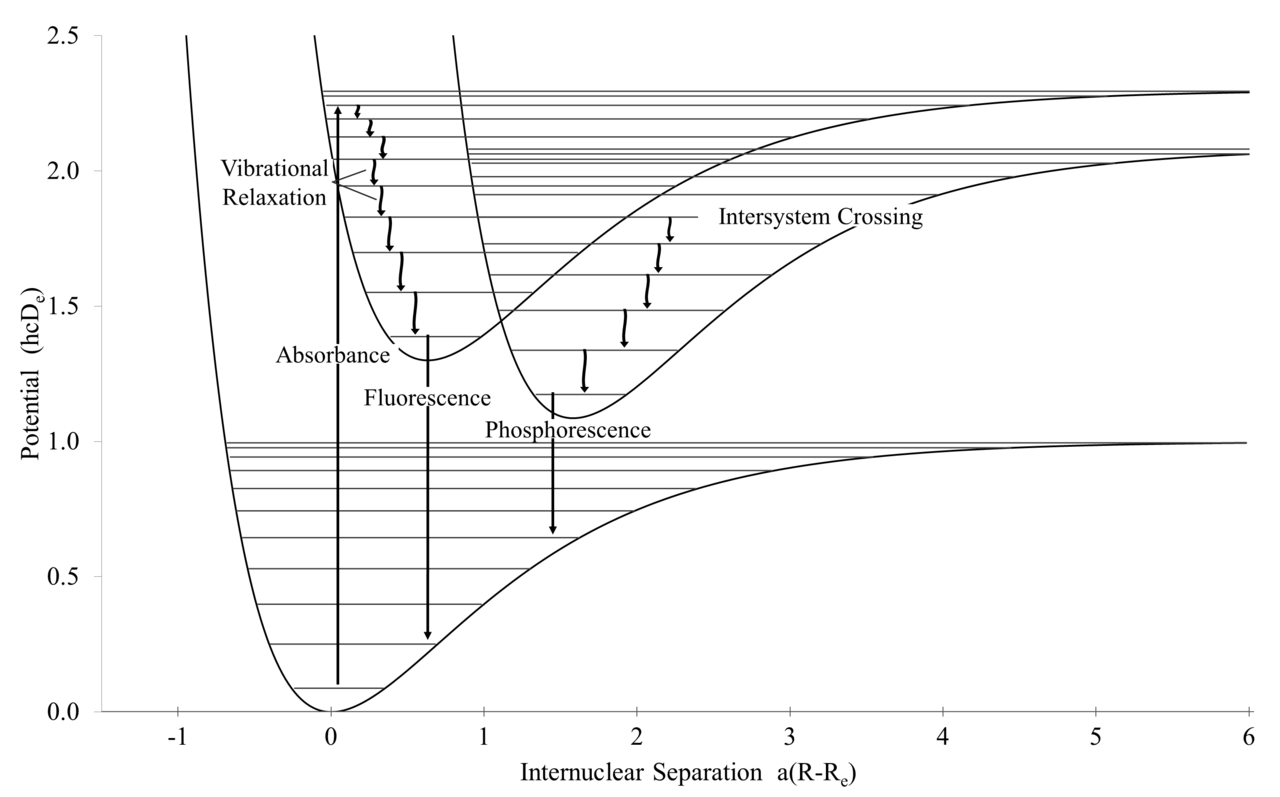
\includegraphics[width=0.85\textwidth]{ISC} 
  \end{center}
  \vspace{-1cm}
  \blfootnote{\tiny Wikipedia, Intersystem Crossing}
\end{frame}

% Motivating example: PHOLEDs
\begin{frame}
  \frametitle{{\bf Ph}osphorescent {\bf O}rganic {\bf L}ight {\bf E}mmitting
  {\bf D}iodes (PHOLED)}
\end{frame}

% Necessary Ingredients
\begin{frame}
  \frametitle{Quantum Mechanical Ingredients for the Treatment of ISC}
  \begin{center}
  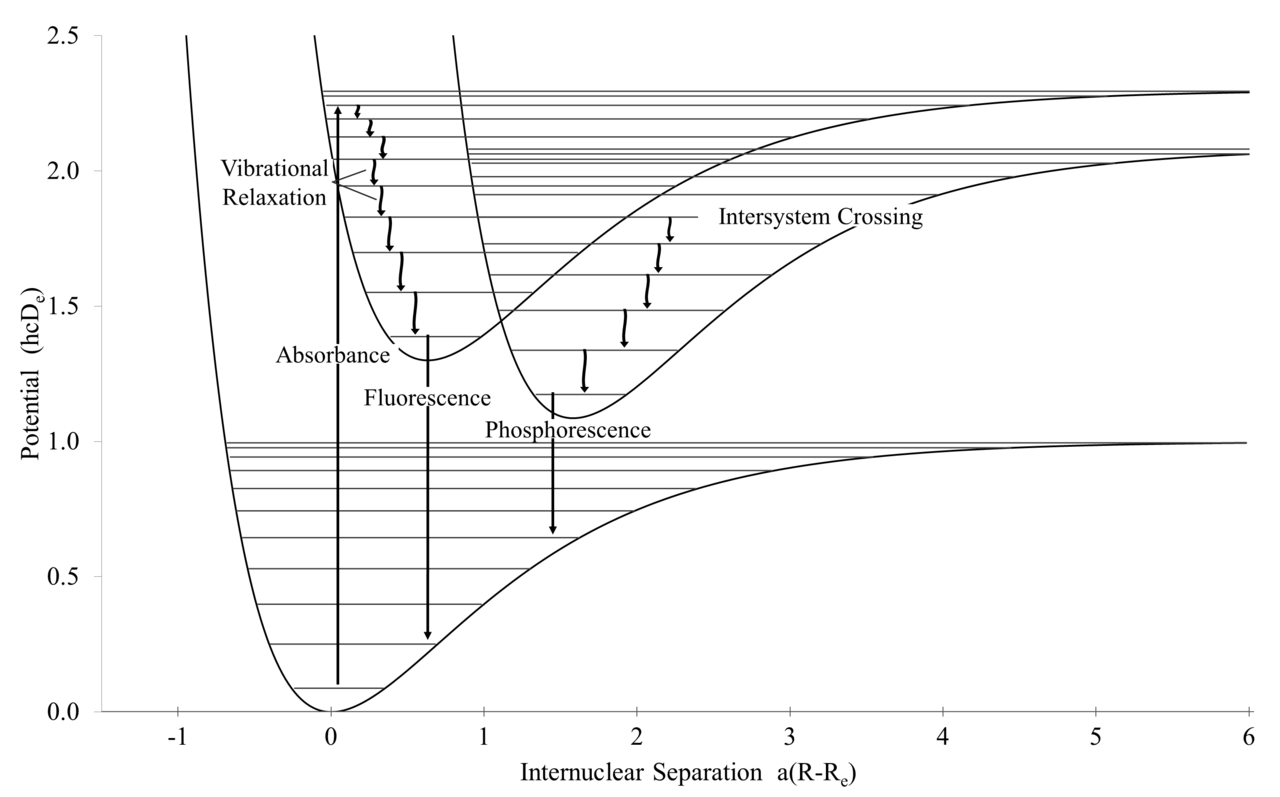
\includegraphics[width=0.7\textwidth]{ISC} 
  \end{center}
  \vspace{-0.5cm}
  A proper quantum mechanical treatment of ISC should include:\\
  \begin{mylist}
    \item Electronic Non--Adiabaticity
    \item Correlated Treatment of Electrons
    \item Proper Treatment of Spin--Orbit Coupling
  \end{mylist}
\end{frame}

% Current state of the art (1)
\begin{frame}
  \frametitle{Current State of the Art \emph{ab initio} Methods for Studying 
  ISC: Trajectory Surface Hopping (TSH)}

  Quantum Mechanically, molecular time--dependence is governed by a Hamiltonian
  wave equation,

  \begin{equation*}
    \bpar{\op{H}_N(t) + \op{H}_{el}(t)} \ket{\Psi (t)} = i\partial_t \ket{\Psi(t)}
  \end{equation*}

  ~\\
  The molecular wave function, $\ket{\Psi(t)}$ formally decomposes into a product
  of electronic and nuclear wave functions

  \begin{equation*} 
    \ket{\Psi (t)} = \ket{\Phi(\vc{R}(t),t)}\otimes\ket{\Theta(t)} 
  \end{equation*} 

  ~\\
  In TSH, we say our nuclei evolve classically
  \begin{equation*}
    \inner{\vc{R}}{\Theta (t)} = \prod_{A = 0}^{N_\mathrm{atoms}} 
    \delta^3(\vc{R} - \vc{R}_A(t))
  \end{equation*}

  \vspace{-0.5cm}
  \blfootnote{\tiny Cederbaum, L.S.; \emph{JCP} \textbf{2008}, 128, 124101}
  \blfootnote{\tiny Adedi, A.; \emph{et. al.}; \emph{PRL} \textbf{2010}, 105, 123002}
\end{frame}

% Current state of the art (2)
\begin{frame}
  \frametitle{Current State of the Art \emph{ab initio} Methods for Studying 
  ISC: Trajectory Surface Hopping (TSH)}

  Working in the basis of adiabatic states,
  \begin{equation*}
    \op{H}(t) \ket{\Psi_I (t)} = E_I(t) \ket{\Psi_I (t)}
    \text{ }\Longrightarrow \text{ }
    \op{H}_{el}(t)\ket{\Phi_I(\vc{R}(t),t)} = 
      \mathcal{E}_I(t)\ket{\Phi_I(\vc{R}(t),t)}
  \end{equation*}
  
  ~\\
  Time--evolution of an electronic superposition state is given by
  \begin{align*}
    &i  \partial_t c_K(t) = H_{KJ}(t) c_J(t) \\
    &H_{KJ}(t) = \delta_{KJ}\mathcal{E}_J(t) - i d_{KJ}^\xi (t) \partial_t R_{\xi}(t) \\
    &d_{KJ}^\xi (t) = \innerop{\Phi_K(\vc{R}(t),t)}{\partial_\xi}{\Phi_J(\vc{R}(t),t)}
  \end{align*}

  \blfootnote{\tiny Tully, J.C., \emph{et. al.}; \emph{JCP} \textbf{1971}, 55, 562}
  \blfootnote{\tiny Tully, J.C.; \emph{Faraday Discuss.} \textbf{1998}, 110, 407}
\end{frame}

% Current state of the art (3)
\begin{frame}
  \frametitle{Current State of the Art \emph{ab initio} Methods for Studying 
  ISC: Trajectory Surface Hopping (TSH)}

  Nuclear position time--evolution is governed by Newton's equations,

  \begin{equation*}
    -\nabla E_c(t) = \vc{m}\cdot \partial_t^2\vc{R}(t)
  \end{equation*}

  ~\\
  The probatility of ``hopping" from the current electronic adiabat to another
  through out the course of a nuclear time--step is given by

  \begin{equation*}
    g_{cK}(t + \Delta t_N) = -2 \int_t^{t + \Delta t_N} 
      \frac{\Re(c_c(t') c^*_K(t'))d_{cK}^\xi (t') \partial_{t'}
      R_{\xi}(t')}{c_c(t') c^*_K(t')}\mathrm{d}t'
  \end{equation*}
  \blfootnote{\tiny Tully, J.C., \emph{et. al.}; \emph{JCP} \textbf{1971}, 55, 562}
  \blfootnote{\tiny Tully, J.C.; \emph{Faraday Discuss.} \textbf{1998}, 110, 407}
\end{frame}

% Treatment of ISC within TSH (1) -- Yes to non--adiabaticity
\begin{frame}
  \frametitle{Treatment of ISC within Trajectory Surface Hopping}
  \begin{center}
  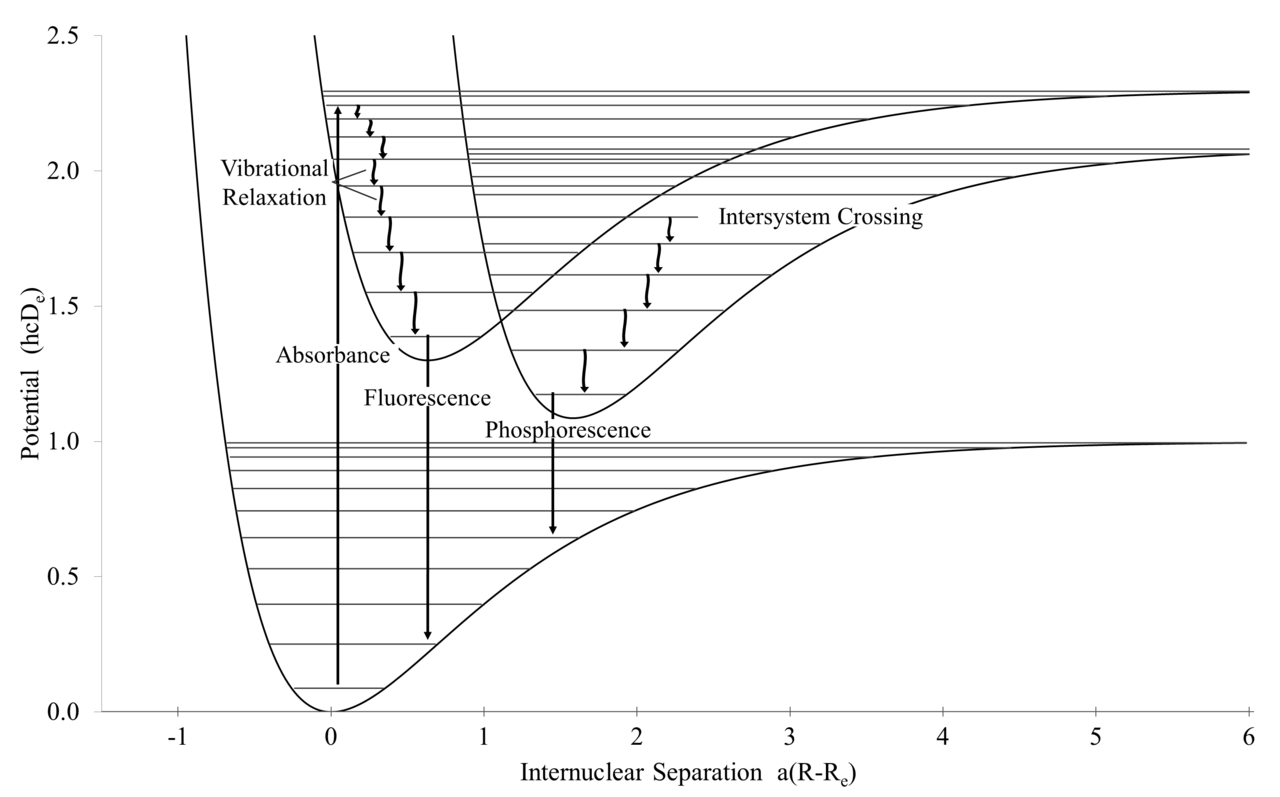
\includegraphics[width=0.7\textwidth]{ISC} 
  \end{center}
  \vspace{-0.5cm}
  TSH treatment of ISC: 
  \begin{mylist}
    \item[\done] Electronic Non--Adiabaticity
    \item Correlated Treatment of Electrons
    \item Proper Treatment of Spin--Orbit Coupling
  \end{mylist}
\end{frame}

% Configuration Interaction (1)
\begin{frame}
  \frametitle{The Configuration Interaction (CI) Method}

  Most implementations of TSH utilize the CI expansion for their description
  of electronic adiabats,
  \begin{align*}
  &\ket{\Phi^N_I (\vc{R}(t),t)} = \sum_{\alpha \in \mathcal{K}^N}  
    \ket{\psi_\alpha (\vc{R}(t),t)} d^I_\alpha(t)
  \\
  & \mathcal{K}^N \subset \left\lbrace \{ \phi_p \} \suchthat \{ \phi_p \} \subset
  \mathcal{R}_0^N \text{ and } \mathrm{card}(\{ \phi_p \}) = N \right\rbrace
  \end{align*}
  
  ~\\
  The expansion coefficients are obtained via diagonalizing the Hamiltonian
  in the basis of Slater determinants
  \begin{align*}
  &H_{\alpha\beta}(t) d_\beta^I(t) = d_\alpha^I(t) \mathcal{E}^N_I(t)
  \\
  &H_{\alpha\beta}(t) =
  \innerop{\psi_\alpha(\vc{R}(t),t)}{\mathcal{H}_{el}(t)}{\psi_\beta(\vc{R}(t),t)}
  \end{align*}
  \blfootnote{\tiny Szabo, A.; \emph{Modern Quantum Chemistry}}
\end{frame}

% Configuration Interaction (2)
\begin{frame}
  \frametitle{The Configuration Interaction (CI) Method}

  The CI expansion is especially simple for TSH as the required entities take on
  very simple forms

  \begin{align*}
    &d_{JK}^\xi = \sum_{\alpha,\beta \in \mathcal{K}^N} 
      \delta_{\alpha\beta} d_\alpha^{J*} \partial_\xi d_\alpha^K +
      d_\alpha^{J*} d_\beta^K 
      \innerop{\psi_\alpha}{\partial_\xi}{\psi_\beta} +
      \mathcal{M}_\mathrm{NAC} \\ \\
    &\nabla \mathcal{E}_J = \sum_{\alpha,\beta \in \mathcal{K}^N} 
      d_\alpha^{J*} d_\beta^J \nabla H_{\alpha\beta} +
      \mathcal{M}_E
  \end{align*}
  \blfootnote{\tiny Yamaguchi, Y.; \emph{et. al.}; \emph{Analytic Derivative Methods in Molecular Electronic Structure Theory: A New Dimension to Quantum Chemistry and its Applications to Spectroscopy}}
\end{frame}

% Treatment of ISC within TSH (2) -- Yes to Correlation 
\begin{frame}
  \frametitle{Treatment of ISC within Trajectory Surface Hopping}
  \begin{center}
  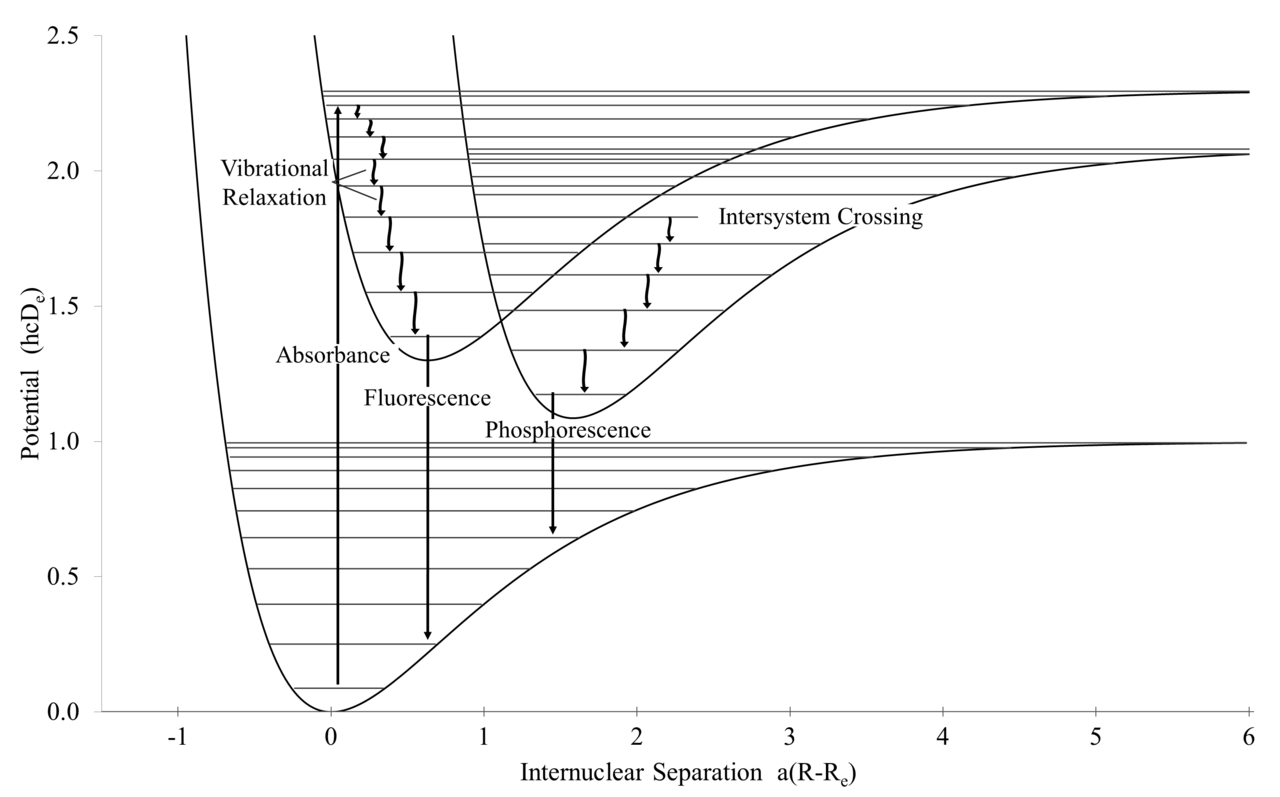
\includegraphics[width=0.7\textwidth]{ISC} 
  \end{center}
  \vspace{-0.5cm}
  TSH treatment of ISC: 
  \begin{mylist}
    \item[\done] Electronic Non--Adiabaticity
    \item[\done] Correlated Treatment of Electrons
    \item Proper Treatment of Spin--Orbit Coupling
  \end{mylist}
\end{frame}

% Relativistic Theory Primer (1)
\begin{frame}
  \frametitle{Relativistic Theory Primer: The (Quasi)--Relativistic Many--Body 
  Molecular Hamiltonian}

  The (quasi)-relativistic many--body molecular Hamiltonian in the absence of 
  an external perturbation may be written (in atomic units) as
  \begin{align*}
%   &\op{H} = \op{H}_N + \op{H}_{el} \\
    &\op{H}_N = \sum_{A=1}^{N_\mathrm{atoms}} \frac{\vc{P}^2_A}{2m_A} \qquad\qquad
     \op{H}^\mathrm{DC}_{el} = 
       \sum_{i=1}^{N_e} h^D(i) + \sum_{i < j}^{N_e} g^C(i,j) + V_{NN} \\
    \\
    & h^D(i) = 
      \begin{pmatrix}
        V_{ne}(\vc{r}_i) && c\text{ }\vc{\sigma} \cdot \vc{p}_i\\
	c\text{ }\vc{\sigma} \cdot \vc{p}_i && V_{ne}(\vc{r}_i) - c^2
      \end{pmatrix} \qquad 
      g^C(i,j) = \frac{1}{\vert \vc{r}_i - \vc{r}_j\vert} + O(c^{-2})
      \\ \\ 
    & V_{ne}(\vc{r}_i) = \sum_{A=1}^{N_\mathrm{atoms}}
                    \int_{\mathbb{R}^3}\mathrm{d}^3\vc{R}
		    \frac{\Gamma_A(\vc{R})}{\vert \vc{r}_i - \vc{R}\vert}
      \qquad V_{NN} = \sum_{A<B}^{N_\mathrm{atoms}}
                    \iint_{\mathbb{R}^3}\mathrm{d}^3\vc{R}\mathrm{d}^3\vc{R}'
		    \frac{\Gamma_A(\vc{R})\Gamma_B(\vc{R}')}
		         {\vert \vc{R} - \vc{R}'\vert}
  \end{align*}
  \blfootnote{\tiny Reiher, M.; \emph{et al}. \emph{Relativistic Quantum Chemistry}}
\end{frame}

% Relativisitc Theory Primer (2)
\begin{frame}
  \frametitle{Relativistic Theory Primer: The (Quasi)--Relativistic Many--Body 
  Molecular Hamiltonian}

  The Dirac--Coulomb Hamiltoninan acts on a 4 dimensional Hilbert space
  known as a bispinor field
  \begin{equation*}
    \op{H}_{el}^\mathrm{DC} \ket{\Phi} \quad \rightarrow \quad 
    \ket{\Phi} = \begin{pmatrix} \ket{\Phi_L} \\ \ket{\Phi_S} \end{pmatrix}
  \end{equation*}
  Of which each L/S component is itself a 2 dimension Hilbert space
  \begin{equation*}
    \ket{\Phi_{L/S}} =
      \begin{pmatrix} \vert\Phi_{L/S}^\alpha\rangle \\ \vert\Phi_{L/S}^\beta\rangle
      \end{pmatrix}
  \end{equation*}
  \blfootnote{\tiny Reiher, M.; \emph{et al}. \emph{Relativistic Quantum Chemistry}}

\end{frame}

% Relativistic Theory Primer (3)
\begin{frame}
  \frametitle{Realivitistic Theory Primer: Effective Two--Component Relativisitc
  Hamiltonian}

  There exists a unitary transformation operator $\op{U}$ such that
  \begin{equation*}
    \op{H}_{el}^\mathrm{DC} \mapsto 
    \begin{pmatrix} \op{H}_{el}^+ && 0 \\ 0 && \op{H}_{el}^- \end{pmatrix} 
    %\qquad
%    \begin{pmatrix} \ket{\Phi_L} \\ \ket{\Phi_S} \end{pmatrix}\mapsto
%    \begin{pmatrix} \ket{\Phi^{2c}} \\ 0 \end{pmatrix}
  \end{equation*}
  This folds the contribution from the small component into the large component 
  \begin{equation*}
    \begin{pmatrix} \ket{\Phi_L} \\ \ket{\Phi_S} \end{pmatrix}\mapsto
    \begin{pmatrix} \ket{\Phi^{2c}} \\ 0 \end{pmatrix}
  \end{equation*}
  \blfootnote{\tiny Reiher, M.; \emph{et al}. \emph{Relativistic Quantum Chemistry}}
\end{frame}

% Relativistic Theory Primer (4)
\begin{frame}
  \frametitle{Realivitistic Theory Primer: Effective Two--Component Relativisitc
  Hamiltonian}

  Expanding the transformed two--component Hamiltonian in the basis of single
  particle Fock states (\emph{molecular orbitals}), we obtain
  \begin{equation*}
    \op{H}_{el} = \sum_{pq}h^\mathrm{2C}_{pq} c_p^\dagger c_q +
    \frac{1}{2}\sum_{pqrs} g_{pqsr}c_p^\dagger c_q^\dagger c_r c_s
  \end{equation*}

  \begin{equation*}
    g_{pqsr} = \iint_{\mathbb{R}^3}\mathrm{d}^3\vc{r} \mathrm{d}^3\vc{r}'
      \frac{\phi^*_p(\vc{r})\phi^*_q(\vc{r}')\phi_s(\vc{r})\phi_r(\vc{r}')}
           {\vert \vc{r} - \vc{r}' \vert} \qquad 
    \phi_p(\vc{r}) = 
      \begin{pmatrix} \phi^\alpha_p(\vc{r}) \\ \phi^\beta_p(\vc{r}) \end{pmatrix}
  \end{equation*}
  \blfootnote{\tiny Reiher, M.; \emph{et al}. \emph{Relativistic Quantum Chemistry}}

\end{frame}

% SOC in TSH currently
\begin{frame}
  \frametitle{Phenomenological Addition of Spin--Orbit Coupling (SOC) in
  Trajectory Surface Hopping}

  Traditionally, SOC is added to nonrelativistic wave functions 
  \emph{a posteriori} in TSH through the SO part of the Dirac--Coulomb
  Hamiltonian
  \begin{equation*}
    h_\mathrm{DC}^\mathrm{SO} (i) = \frac{1}{2c^2} \sum_{A=1}^{N_\mathrm{atoms}}
      \int_{\mathbb{R}^3}\mathrm{d}^3\vc{R}
      \frac{\Gamma_A(\vc{R})
        (( \vc{r}_i - \vc{R} ) \times \vc{p}_i)\cdot \vc{s}_i}
	{\vert \vc{r}_i - \vc{R} \vert^3}
  \end{equation*}

  This yields an extraneous coupling in the electronic equations of motion

  \begin{equation*}
    H_{KJ} = \delta_{KJ}\mathcal{E}_J(t) +
    {\color{red}
      \innerop{\Phi_K(\vc{R}(t),t)}{\mathcal{H}_{SO}^{DC}}{\Phi_J(\vc{R}(t),t)}
    }
    - i d_{KJ}^\xi (t) \partial_t R_{\xi}(t) 
  \end{equation*}
  \blfootnote{\tiny Chang, A.H.H.; \emph{JCP} \textbf{1993} 99, 6824}
  \blfootnote{\tiny Daniel, C.; \emph{JCP} \textbf{1997} 106, 1421}
\end{frame}

% Treatment of ISC within TSH (3) -- No to SOC 
\begin{frame}
  \frametitle{Treatment of ISC within Trajectory Surface Hopping}
  \begin{center}
  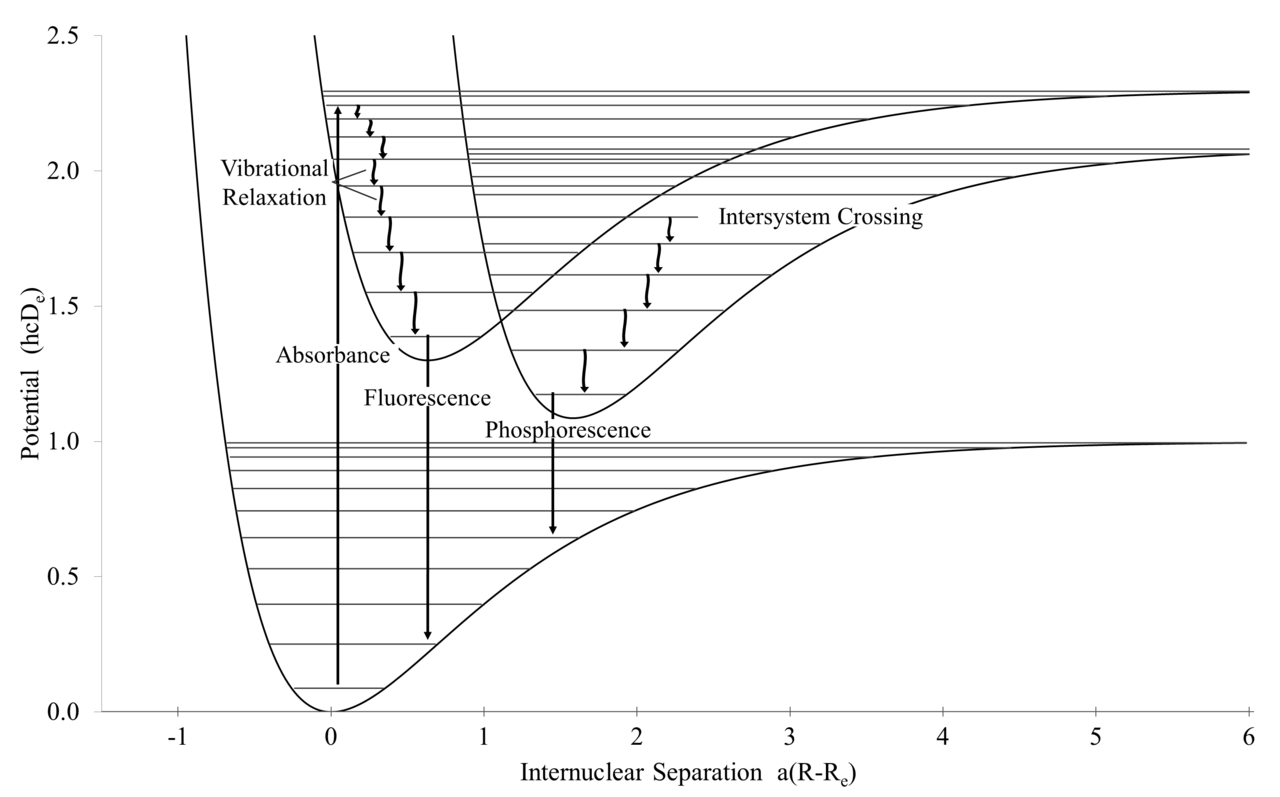
\includegraphics[width=0.7\textwidth]{ISC} 
  \end{center}
  \vspace{-0.5cm}
  TSH treatment of ISC: 
  \begin{mylist}
    \item[\done] Electronic Non--Adiabaticity
    \item[\done] Correlated Treatment of Electrons
    \item[\wontfix] Proper Treatment of Spin--Orbit Coupling
  \end{mylist}
\end{frame}

% How we're going to solve it with relativistic surface hopping dynamics
\begin{frame}
  \frametitle{Solution: Relativistic Non--Adiabatic Molecular Dynamics}

  To properly account for SOC in TSH, each of the electronic adiabats must
  be mutually optimized under a relativistic Hamiltonian

  \begin{equation*}
    d_{JK}^\xi \propto \frac{\innerop{\Phi_I}{(\partial_\xi \mathcal{H})}{\Phi_J}}{\mathcal{E}_K - \mathcal{E}_J}
  \end{equation*}
  ~\\
  ~\\
  ~\\

  SOC couples the adiabatic states through the non--adiabatic coupling

  \begin{equation*}
    \partial_\xi \mathcal{H}^{DC} \leftarrow \partial_\xi \mathcal{H}^{DC}_\mathrm{SO}
  \end{equation*}

  and thus enters into the expression for the hopping probablity.
\end{frame}


% Previous Work
\begin{frame}
  \frametitle{Previous Work towards Relativistic Non--Adiabatic Molecular Dynamics}
\end{frame}

% pp-TDA
\begin{frame}
  \frametitle{The Particle--Particle Tamm--Dancoff Approximation (pp--TDA)}
  
  In the pp-TDA, the $N$-electron ground and excited states may be written as two
  particle additions to an $(N-2)$-electron reference determinant,
  \begin{equation*}
    \ket{\Phi_I^N (\vc{R}(t),t)} = \sum_{a < b} X_{ab}^I(\vc{R}(t),t)
    c_a^\dagger(\vc{R}(t)) c_b^\dagger (\vc{R}(t))
    \ket{\psi_0^{(N-2)}(\vc{R}(t),t)}
  \end{equation*}

  which may we written as a CI expansion
  \begin{equation*}
    \mathcal{K}_\mathrm{pp-TDA}^N =
    \left\lbrace \{ \phi_p \}^{(N-2)}_0 \cup \{\phi_a,\phi_b \} \suchthat 
    \{ \phi_a,\phi_b \} \subset \mathcal{R}^{(N-2)}_0 \setminus \{\phi_p \}^{(N-2)}_0 
    \right\rbrace
  \end{equation*}

  This yields the Hamiltonian eigenproblem,
  \begin{align*}
    &\sum_{c < d} A_{ab,cd} X_{cd}^I = \omega'_I X_{ab}^I \quad (a < b) \qquad
    &A_{ab,cd} = \delta_{ac}\delta_{bd}(\varepsilon_a + \varepsilon_b) + 
      \innerop{ab}{}{cd}
  \end{align*}
  \begin{align*}
    &\omega'_I = \mathcal{E}^{N}_I - \mathcal{E}^{(N-2)}_0
  \end{align*}
  \blfootnote{\tiny Yang, Y.; \emph{et al.}; \emph{JCP} \textbf{2013} 139, 224105}
\end{frame}

% pp-X2C (1)
\begin{frame}
%  \frametitle{The Relativistic Particle--Particle Tamm-Dancoff Approximation 
%  (X2C--pp--TDA)}
  \begin{center}
    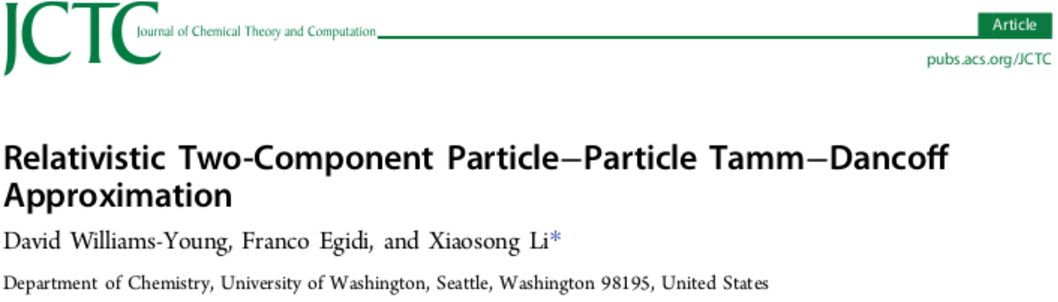
\includegraphics[width=\textwidth,height=0.32\textheight]{ppX2CTop} 

    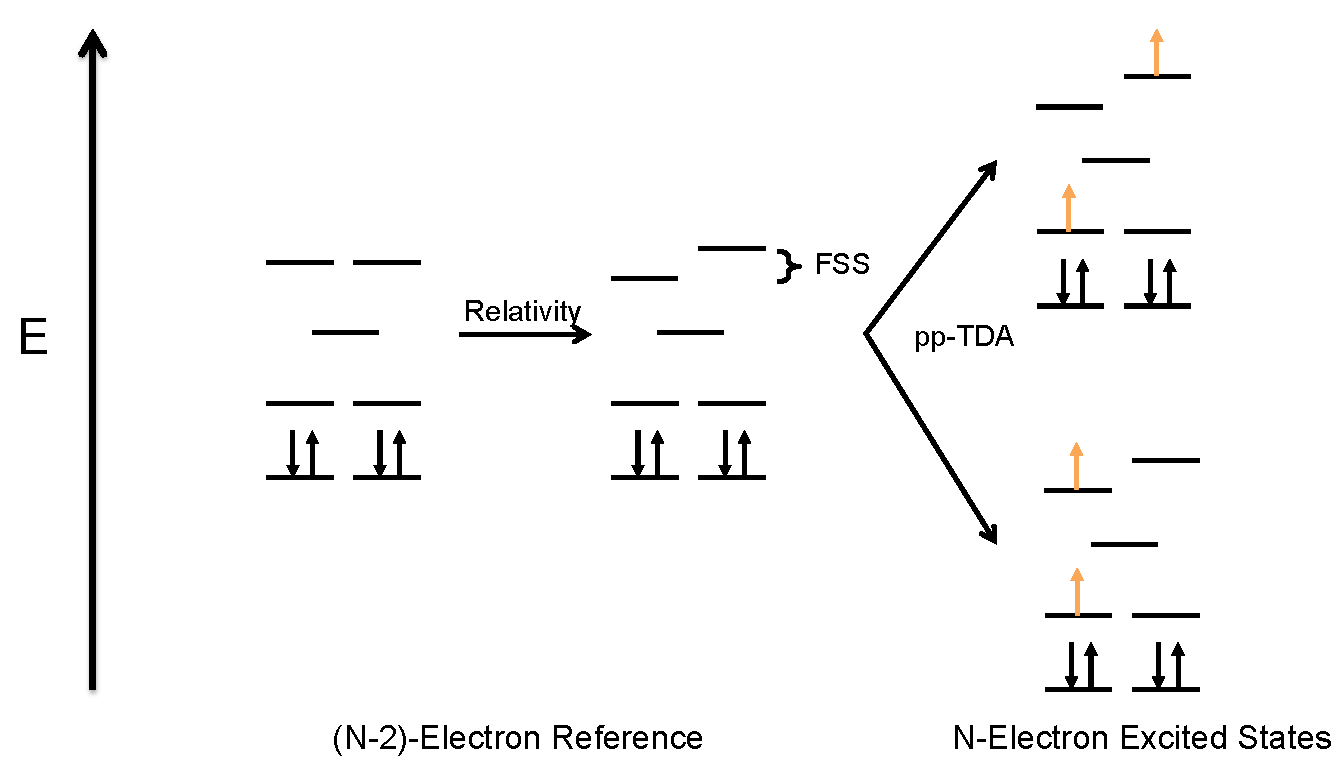
\includegraphics[width=0.8\textwidth]{ppX2C_TOC} 
  \end{center}
\end{frame}

% pp-X2C (2)
\begin{frame}
  \frametitle{The Relativistic Particle--Particle Tamm-Dancoff Approximation 
  (X2C--pp--TDA)}
  {\scriptsize
  \begin{table}
    \centering
    \begin{tabular}{llll}
    System                    & Level                              & pp-TDA & Ref\\
    \hline
    \multirow{4}{*}{Mg}        & $^3$P$^\circ_{1}-^3$P$^\circ_{0}$  & 2.77  & 2.49 \\
                               & $^3$P$^\circ_{2}-^3$P$^\circ_{1}$  & 5.55  & 5.05 \\
                               & $^3$P$^\circ_{1}-^3$P$^\circ_{0}$  & 0.42  & 0.41 \\
                               & $^3$P$^\circ_{2}-^3$P$^\circ_{1}$  & 0.84  & 0.84 \\
    \hline
    \multirow{4}{*}{Al$^+$}    & $^3$P$^\circ_{1}-^3$P$^\circ_{0}$  & 9.13   & 7.55  \\
                               & $^3$P$^\circ_{2}-^3$P$^\circ_{1}$  & 18.40  & 15.36 \\
                               & $^3$P$^\circ_{1}-^3$P$^\circ_{0}$  & 2.17   & 1.73  \\
                               & $^3$P$^\circ_{2}-^3$P$^\circ_{1}$  & 4.50   & 3.65  \\
    \hline
    \multirow{4}{*}{Si$^{2+}$} & $^3$P$^\circ_{1}-^3$P$^\circ_{0}$  & 18.97  & 15.94 \\
                               & $^3$P$^\circ_{2}-^3$P$^\circ_{1}$  & 38.40  & 32.45 \\
                               & $^3$P$^\circ_{1}-^3$P$^\circ_{0}$  & 5.08   & 4.10  \\
                               & $^3$P$^\circ_{2}-^3$P$^\circ_{1}$  & 11.04  & 9.07  \\
    \hline
    \end{tabular} $\quad$
    \begin{tabular}{llll}
    System                    & Level & pp-TDA & Ref\\
    \hline
     O$_2$ & $^3\Delta_3-{^3\Delta_2}$ & 20.58 & 18.09 \\ \hline
     \multirow{2}{*}{Al$^+$} & $^3$P$_1-^3$P$_0$ & 9.20 & 7.75 \\ 
     & $^3$P$_2-^3$P$_1$ & 17.93 & 15.03 \\  \hline
     \multirow{2}{*}{Si$^{2+}$} & $^3$P$_1-^3$P$_0$ & 19.46 & 16.55 \\ 
     & $^3$P$_2-^3$P$_1$ & 37.88 & 32.06 \\    \hline
    \end{tabular}
  \end{table}
  }
  \blfootnote{\tiny DBWY, Egidi, F.; Li, X.; \emph{JCTC} \textbf{2016} Just Accepted}
  \blfootnote{\tiny Kramida, A.; \emph{et al.}; \emph{NIST Atomic Spectra Datapage}}
\end{frame}

\begin{frame}
  \frametitle{Trajectory Surface Hopping within the pp--TDA}
  \vspace{-0.7cm}
  \begin{figure}
  \begin{subfigure}[b]{0.40\textwidth}
  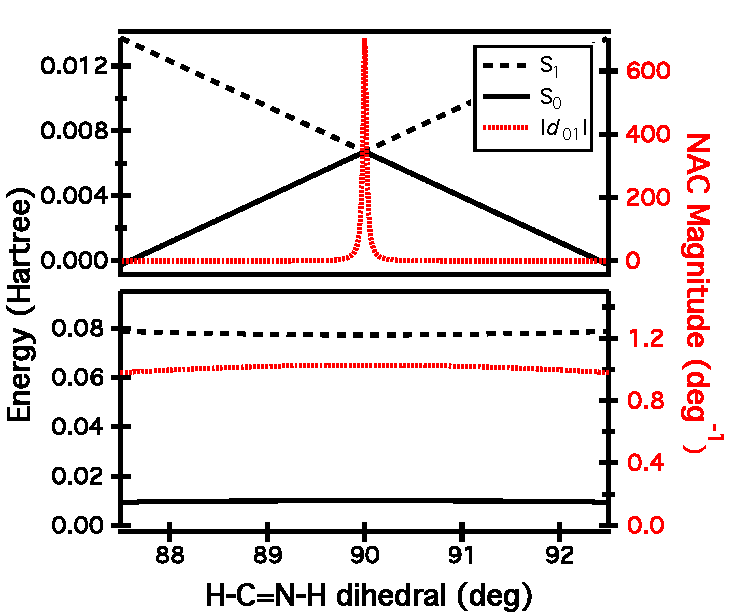
\includegraphics[width=\textwidth]{gs_es_dercp} 
  \caption{ }
  \label{fig:gs_es_dercp}
  \end{subfigure} $\quad$
  \begin{subfigure}[b]{0.40\textwidth}
  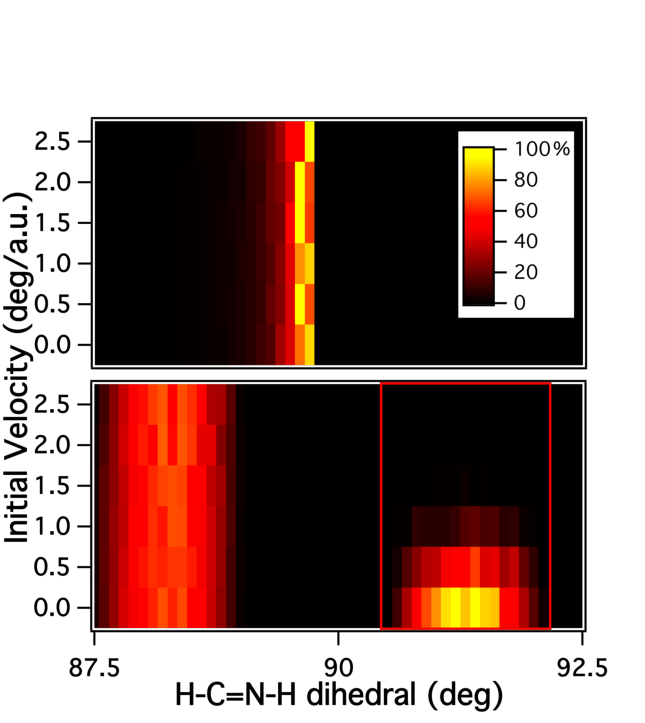
\includegraphics[width=\textwidth]{stacked_hops} 
  \caption{ }
  \label{fig:hops}
  \end{subfigure}
  \vspace{-0.4cm}
  \caption{\tiny \footnotesize (a) Potential energy surfaces for ground and excited
  states, and the coupling strength between the two states with respect to the
  dihedral angle in the vicinity of the minimum energy crossing point between
  S$_0$ and S$_1$ from the pp-TDA (top frame) and CIS (bottom frame) approaches.
  (b) Color maps showing the distribution of configurations at which hops from
  S$_1$ to S$_0$ occur for the different initial velocities resolved at the
  pp-TDA (top frame) and CIS (bottom frame) levels of theory (area in red box
  magnified, after normalization, 1000$\times$ for visibility.)}
  \end{figure}
\end{frame}
\end{document}
